\chapter{Software Design, Implementation and Testing}

\section{Design}

\subsection{Tool Selection }

\subsubsection{Programming Language}

This project is focused on algorithm design and the performance of this algorithm therefore I wanted a language that was rich in features but capable of high performance. The language needed to support object orientation and the necessary data structures that will aid in its implementation. Python, C++ and Java were all languages that I considered. I also wanted a language that had access to a huge amount of libraries so that I could leverage these resources to more quickly and efficiently create my project, Python fulfills this requirement more than the others. I also wouldn't need to create a web or GUI interface both of these are areas that Java is especially good at with the JavaFX library providing an easy way to implement graphical elements and the Spring package providing an easy way to create API calls for a web interface. Python and Java are slower than C++\cite{java_vs_c++}\cite{c++_vs_python} with Python being significantly slower. C++ is the better choice in terms of efficiency however I'm not aiming to create the fastest TSP solver only compare results so the speed benefit may not be required. C++ is also a less forgiving language where it's easier to make mistakes, if I wanted to use C++ then I would have had to spend a long time learning C++ in finer detail. 

I also wanted to be able to prototype solutions and due to Python's console support it is the language that would allow me to do this in the quickest and most efficient manner. With this in mind and its huge amount of library support especially in the area of data science/AI Python ended up being the better choice for me. 

\subsubsection{Development Environment}

I used the IntelliJ IDE PyCharm for this project\cite{pycharmide}, this IDE is easy to use but provides complex features that prove very useful, these features include; refactoring tools, Thread concurrency monitoring, automated Unit testing tools and automated Virtualenv creation. I developed on linux 

\subsubsection{Version Control System}
I used GitHub\cite{github} to host the code for my project and act as a Version Control System (VCS). This allowed for me to keep a backup of all the work I had done so if I needed to refer back to a change I'd made previously it was there and easy to access. GitHub is also really easy to setup and access and it can be connected to other applications for services like Continuous Integration.

\subsection{Overall Architecture}

My research required a piece of software be designed and built that could:

\begin{itemize}
    \item Load in TSP files
    \item Run the selected clustering algorithms over this data
    \item Run ACO over this clustered data
    \item Create a way to travel from one cluster to another in the tour
    \item Run a tour finding algorithm on the nodes inside each cluster
    \item Calculate the length of the tour
    \item Plot graphs relating to the tour
    \item Be able to execute the program as a script with CLI arguments
\end{itemize}

Based off of this I created a list of requirements, these are in Appendix \ref{appendix_requirements}. These were created at the start of the program and because I was using an Agile approach weren't kept fully up to date but represent my thoughts about the software when I started building it which was a couple of weeks into the project.

My program works by:
\begin{enumerate}
    \item Loading in the data, this is stored as a TSPLIB95 file.
    \item Then clustering this and storing the clustered data.
    \item Run an ACO algorithm over the clusters to form a tour.
    \item Turning the ACO tour into a local tour by finding the entry and exit nodes for each cluster. These are the nodes that are closest to the next cluster in the tour.
    \item Find a tour through each of the clusters the tour starts at the entry node and ends at the exit node. This tour then gets recorded.
    \item Build a global tour by following through the ACO tour and substituting the clusters for the tours that were found in each cluster
    \item Run 2-opt over that tour
    \item Plot all the graphs
\end{enumerate}

The output of the program gets saved to a log file for future reference.

I wanted to be able to create my own TSP data this was because there wasn't a huge amount of small TSP data. Lots of it was several thousand nodes in size and I wanted to test my algorithm on problems containing hundreds of nodes because it would have taken too long to tests on these very large multi-thousand node problems.

\subsubsection{Automated DBSCAN eps}

One of the areas that I was keen to improve on was the clustering, whilst I couldn't create a brand new clustering algorithm I did manage to automate a way to improve upon DBSCAN. As I mentioned previously DBSCAN requires a parameter called eps this is what allows for clusters to be found and is the most important factor to choose when using the Algorithm. In \cite{optimal_eps_value_DBSCAN} Rahmah and Sitanggang figure out a way to find this value using a nearest neighbours approach.

\begin{figure}[h]
    \centering
    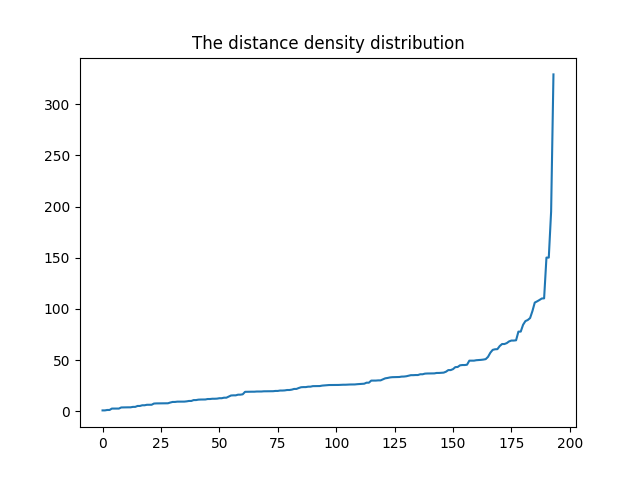
\includegraphics[width=\textwidth]{figures/eps_finder_graph_whole.png}
    \caption{Figure showing the graph that gets plotted when you find the distance from one node to every other.}
    \label{fig:whole_eps_graph}
\end{figure}

\begin{figure}[h]
    \centering
    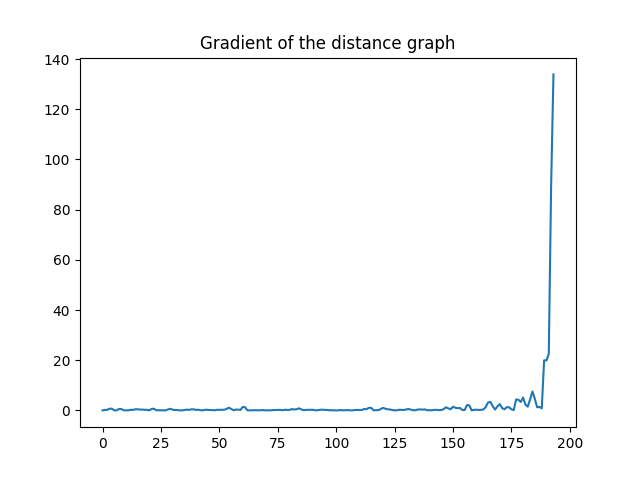
\includegraphics[width=\textwidth]{figures/eps_finder_graph_gradient.png}
    \caption{Figure showing the graph that gets plotted when you find the gradient of the nearest neighbour distances, this is the gradient of the graph shown in figure \ref{fig:whole_eps_graph}.}
    \label{fig:gradient_eps_graph}
\end{figure}

\begin{figure}[h]
    \centering
    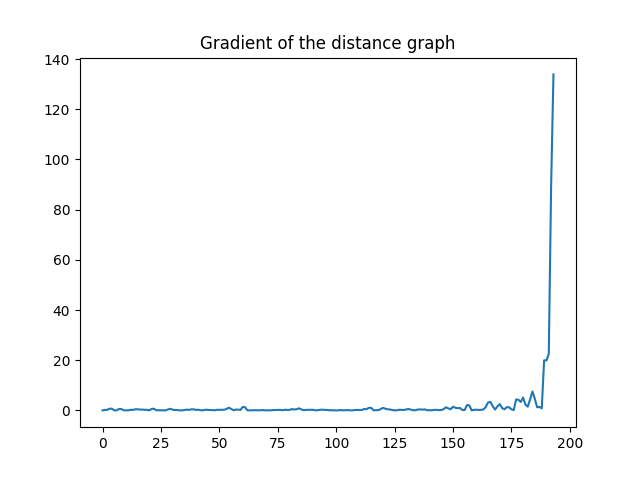
\includegraphics[width=\textwidth]{figures/eps_finder_graph_gradient.png}
    \caption{Figure showing the graph that gets plotted when you remove the last 1/7th of the data from the graph shown in figure \ref{fig:whole_eps_graph}.}
    \label{fig:cut_eps_graph}
\end{figure}

Their approach consisted of finding the distance between one node and all other nodes and then plotting these distances as a graph. This graph can be seen in figure \ref{fig:whole_eps_graph}, the optimal eps value is when the graph starts to curve. 

This can be found using the Nearest Neighbours algorithm present in Scikit Learn\cite{scikit_learn_nearest_neighbours}. To find the turning point of the graph I tried to take take the derivative and find where the change was biggest figure the graph of this is shown in figure \ref{fig:gradient_eps_graph}. This approach didn't work because if I were to take the largest gradient then I would end up with the eps value being the largest distance between two nodes which would result in DBSCAN finding a cluster that contained every node. To get around this I cut the last 1/7th off the graph and then found the highest point this graph is shown in figure \ref{fig:cut_eps_graph}. This approach worked for every piece of data that I tested it on however there may be data where this wouldn't work such as where the data increases in a circle out from central point.

\subsubsection{Script Interface}

I needed to create an easy way to run my program that would allow me to setup all my experiments and run them through quickly, I thought about using an web interface or building a GUI for this that would allow runs to be queued up and executed when the previous one had finished but I decided against this because I thought that it would be over complicate things and instead I wanted to focus on the research side, instead I made it execute like a script. A script allows for queuing tasks up to be ran and would be easier to implement so would give me more time to focus more on the experiments to be ran.

The program is constructed to allow for command line arguments to be given, these are available in Table \ref{tab:commandargs} in Appendix \ref{apd:commandline_arguments}. The arguments allow for every aspect of the program to be controlled such as; the arguments provided to the clustering algorithms and the ACO algorithms, the input file to read, output folder, the clustering and ACO algorithms to use and it allows for various features to be turned on or off. 

Not all of these parameters have to be given every time you run the program only a few are essential and the parameters that are optional and aren't set are auto-populated from a list of default values, these default values are also shown in the table.

To hold these options values I had an Options class, this made use of pythons ability to have function arguments hold default values, when this class was constructed all the command line arguments were passed to it and the ones that weren't provided were taken from the default values file.

\section{Implementation}

There are several key sections to my project, this section discusses the implementation of them, I made use of existing libraries in my project to speed up the work and allow me to focus more on the research. Some of these libraries needed changes so they worked the way I wanted them to and so they had all the features I needed. 

\subsection{Loading TSP Files}

As I mentioned previously I'm using common TSPLIB files these files can hold a lot of data and creating a parser that can deal with all of that would be a tremendous amount of work. I found the library tsplib95\cite{tsplib95} this can read in all sorts of TSPLIB files and works very well. This library contains lots of helpful utility functions that I thought may be useful, features such as: turning the problem into a networkx\cite{networkx} graph and creating distance matrices for the data.

When the file gets loaded in I turn it into a numpy\cite{numpy} array, it has to be a numpy array in order to work with the clustering algorithms. 

\subsubsection{Generating TSP Data}


\subsection{Clustering}

The clustering algorithms that I wanted to implement were all available as part of the Scikt Learn library. In order to use this the data had to be available as a numpy array so I had to ensure that when I read the data in I transformed in into an array. 

When the data gets clustered I needed a way to hold all the data for this I made two classes one called ClusteredData and the other called Cluster. ClusteredData holds all the nodes in the problem and all the clusters that have been created, there are two sorts of clusters that it can hold: full clusters and unclassified node clusters. Some of the clustering algorithms return nodes that don't fit into any specific cluster so I call these unclassified node clusters, these are treated differently because they don't need a tour created for them or entry/exit nodes calculated. 

\subsection{Graph Plotting}

I used the library Matplotlib\cite{matplotlib} to do all my graph plotting, it's very feature rich and allowed me to easily create graphs so made sense for me to use it instead of creating my own plotting library. The graphs are plotted at the end of the run so as not to slow down the program and interfere with the run time statistic.

The following graphs are plotted:

\begin{itemize}
    \item ACO tour of the clustered data
    \item All the nodes in the problem
    \item The data after it had been clustered
    \item The tour for each cluster
    \item The final tour before 2-opt
    \item The final tour after 2-opt
\end{itemize}

\subsubsection{Visualiser of 2-opt and ACO Tour Improvements}

In addition to the graphs that get plotted two videos are also created one that shows the incremental improvement that 2-opt makes and another that shows the incremental improvement of ACO. This works by having a class called TourImprovementAnimator that both 2-opt and ACO have a reference to, every time there is an improved tour they record this on the object.

At the end of the program when the solution has been found the graphs get plotted. The TourImprovementAnimator plots all the tours and saves them to a folder using Matplotlib\cite{matplotlib}. This plotting makes use of the Python multiprocessing library which greatly speeds this process up, these images are then read back in and placed into a video using the library imageio\cite{imageio}.

\subsection{ACO}

I have used two ACO libraries; ACOPY\cite{acopy} and an ACO algorithm that makes use of multi-threading\cite{multithreaded_aco}. ACOPY was available as a dependency that I could install via pip, the other one was not and so I had to pull the code from its GitHub repository and use it that way. The code was meant to be ran on Python 2 and since I was using Python 3 I had to make some small changes to it in order to get it to work, these were mostly upgrading the tests and changing some parameters to be lists. 

ACOPY allowed you to add plugins to extend the functionality of the algorithm. The plugins get called at various points and allow for changes to be made to various parts of the algorithm. I created two plugins the first one records data about the current iteration including the tour and the length of this tour, the second one records the tour after every iteration into a TourImprovementAnimator object.

The other library doesn't have plugin functionality or anything similar so I had to modify the code to get it to print out the data after every iteration and record the tour into a TourImprovementAnimator.

I implemented the second library because when I was running ACOPY I noticed that it took a while to run and only used one core so I found the multi-threaded ACO algorithm to see if it helped speed the program up

\subsection{2-opt}

2-opt is a simple local search algorithm it can be seen as a way to smooth out a tour by deleting crossed over paths, this can be seen in figure \ref{fig:2-opt-example}. 2-opt works by removing two edges from the tour and reconnecting them, it only does this if the resultant tour will be shorter. The pseudo code is shown in Figure \ref{fig:2-opt-epseudo-code}.

\begin{figure}[h]
    \centering
    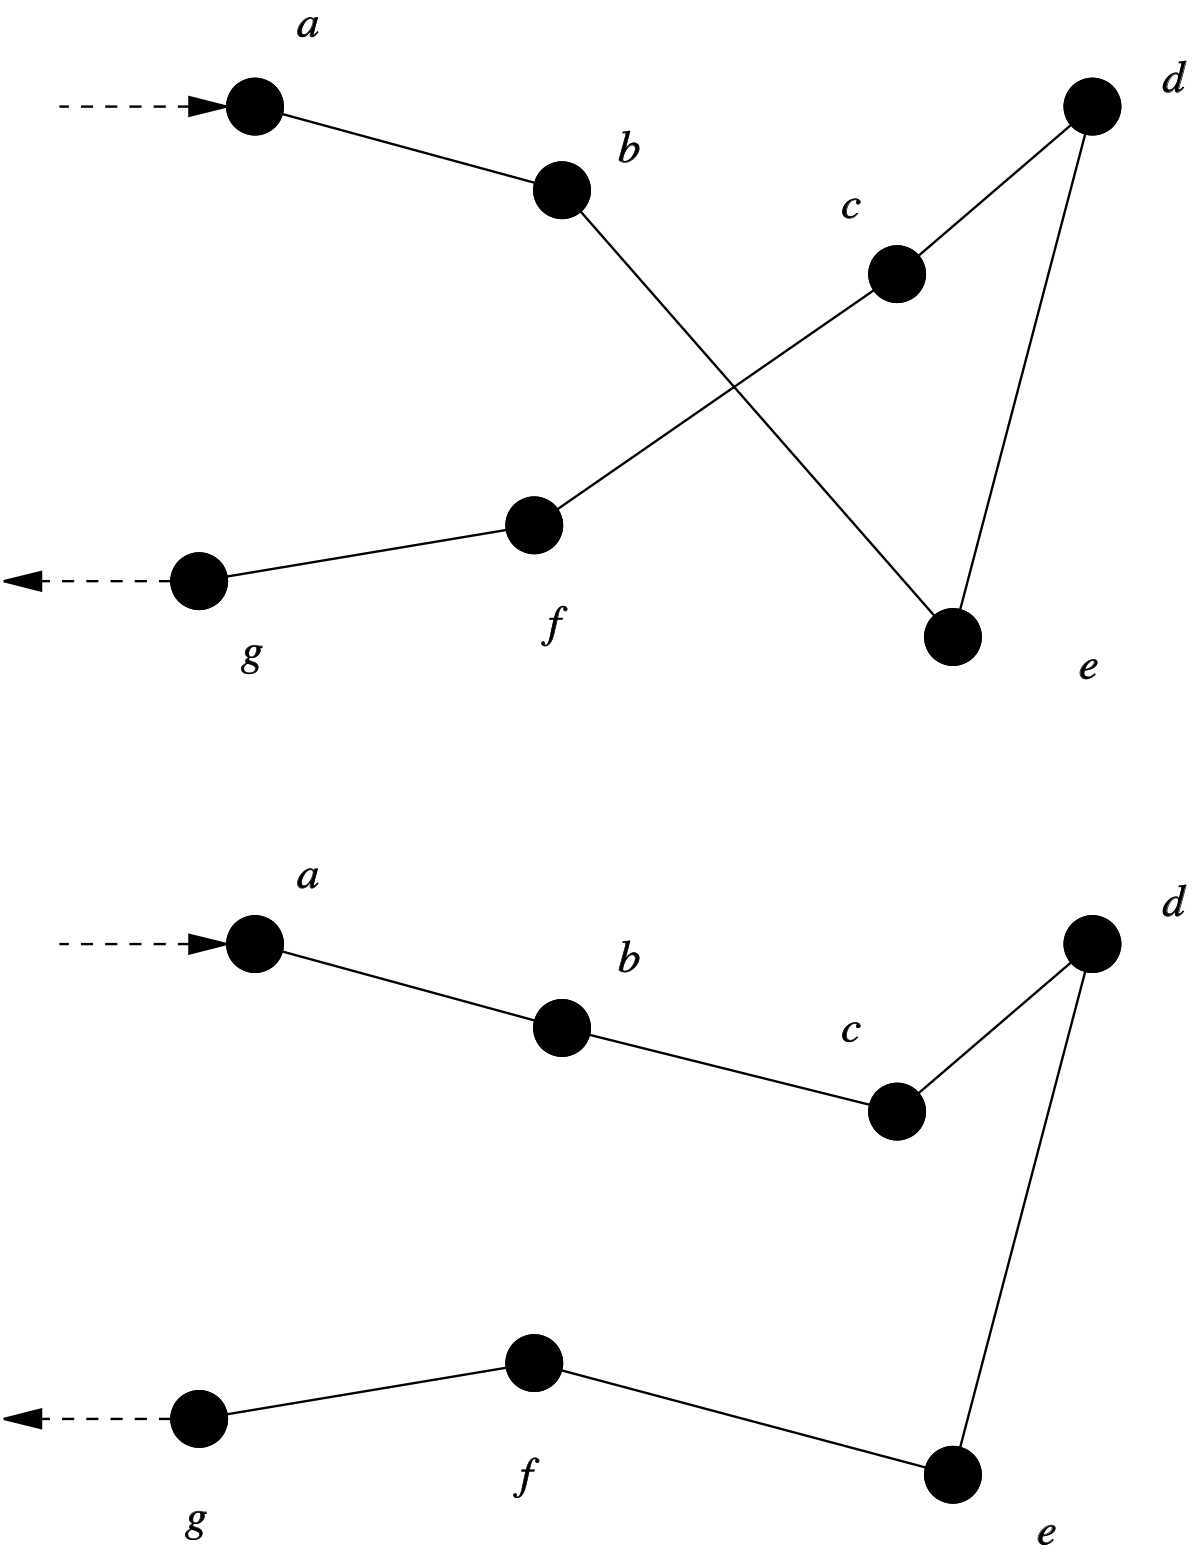
\includegraphics[width=\textwidth]{figures/2-opt-example.png}
    \caption{An example of 2-opt running over a tour. It has swapped the connection b-e and f-c which has removed the cross and made the tour shorter.\cite{2_opt_example_picture}}
    \label{fig:2-opt-example}
\end{figure}

\begin{figure}[h]
    \centering
    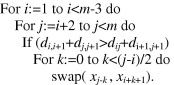
\includegraphics[width=\textwidth]{figures/2_opt_pseudo_code.jpg}
    \caption{The pseudo code for the 2-opt local search algorithm.\cite{2-opt_pseudo_code}}
    \label{fig:2-opt-epseudo-code}
\end{figure}

My implementation is modified slightly because a TourImprovementAnimator records the tour each time an improvement is found.

The run time of 2-opt is quite high and it could be improved through the use of multi-threading but I was unable to do this and couldn't find any references to it online when I looked.

\subsection{Tours Within Clusters}

When the ACO tour over the clustered data has finished I needed a way of turning the ACO tour into a tour that covered every node. The first thing that happens here is the nodes to move from one cluster to the next are found. These are called the entry and exit nodes and are found by finding the two closest nodes between each cluster. 

Tours are then found in every cluster going from the entry node to the exit node, these tours can be found by using ACO and by using a greedy nearest neighbour heuristic. The ACO approach uses the ACO algorithm that the user has specified, when this is used the end node is not included in the ACO search this is because the ACO algorithm has no way to specify the end node. To get around this I add the end node on when the search has finished however this can cause bad unoptimised tours.

The heuristic approach works by starting at the clusters entry node and travelling to the nearest node that it hasn't previously visited and travelling to the exit node last.

\section{Testing}


\subsection{Overall Approach to Testing}

I wanted as much automated testing as possible because I find it is incredibly useful to be able to test your software every time a change is made. This really allows you to be confident in the changes you are making. Due to the complicated nature of my project and the amount of time that is required for a run to successfully take place I knew that not everything would be able to be testing in this fashion.

I utilised quite a lot of informal testing every time a new change was made I ran the code through and ensured that everything was working as it should.

\subsection{Automated Testing}

I used the continuous integration platform Travis-CI\cite{travis_ci} to automatically run my tests. Travis links to your GitHub profile and when you a new commit is pushed it starts a build process. It reads a configuration file located in the root of the repository called .travis.yml which contains all the build instructions. My file told Travis that Python was being used, to install the requirements listed in requirement.txt and run the tests using pytest. If the tests passed then the build was successful otherwise the build failed and I was notified. 

The automated tests I wrote focused on loading in data and the ClusteredData class, lots of tests were also provided from the multithreaded ACO algorithm which I included.

